\documentclass{article}
\RequirePackage{amsmath}
\RequirePackage{bytefield}
\RequirePackage{graphicx}
\RequirePackage{newtxmath}
\RequirePackage{mathtools}
\RequirePackage{xspace}
\RequirePackage{url}
\RequirePackage{changepage}
\RequirePackage{lmodern}

\setlength{\oddsidemargin}{-0.25in} % Left margin of 1 in + 0 in = 1 in
\setlength{\textwidth}{7in}   % Right margin of 8.5 in - 1 in - 6.5 in = 1 in
\setlength{\topmargin}{-.75in}  % Top margin of 2 in -0.75 in = 1 in
\setlength{\textheight}{9.2in}  % Lower margin of 11 in - 9 in - 1 in = 1 in
\setlength{\parskip}{1.5ex}
\setlength{\parindent}{0ex}

\mathchardef\mhyphen="2D

\RequirePackage[usenames,dvipsnames]{xcolor}
% https://en.wikibooks.org/wiki/LaTeX/Colors#The_68_standard_colors_known_to_dvips
\newcommand{\eli}[1]{{\color{JungleGreen}\sf{Eli: #1}}}
\newcommand{\sean}[1]{{\color{blue}\sf{Sean: #1}}}
\newcommand{\taylor}[1]{{\color{red}\sf{Taylor: #1}}}
\newcommand{\daira}[1]{{\color{RedOrange}\sf{Daira: #1}}}
\newcommand{\nathan}[1]{{\color{ForestGreen}\sf{Nathan: #1}}}
\newcommand{\todo}[1]{{\color{Sepia}\sf{TODO: #1}}}

\newcommand{\changedcolor}{magenta}
\newcommand{\setchanged}{\color{\changedcolor}}
\newcommand{\changed}[1]{{\setchanged{#1}}}

% terminology

\newcommand{\term}[1]{\textsl{#1}\xspace}
\newcommand{\termbf}[1]{\textbf{#1}\xspace}
\newcommand{\conformance}[1]{\textmd{#1}\xspace}

\newcommand{\Zcash}{\termbf{Zcash}}
\newcommand{\Zerocash}{\termbf{Zerocash}}
\newcommand{\Bitcoin}{\termbf{Bitcoin}}
\newcommand{\ZEC}{\termbf{ZEC}}
\newcommand{\zatoshi}{\term{zatoshi}}

\newcommand{\MUST}{\conformance{MUST}}
\newcommand{\MUSTNOT}{\conformance{MUST NOT}}
\newcommand{\SHOULD}{\conformance{SHOULD}}
\newcommand{\SHOULDNOT}{\conformance{SHOULD NOT}}
\newcommand{\MAY}{\conformance{MAY}}

\newcommand{\coin}{\term{coin}}
\newcommand{\coins}{\term{coins}}
\newcommand{\coinCommitment}{\term{coin commitment}}
\newcommand{\coinCommitments}{\term{coin commitments}}
\newcommand{\coinCommitmentTree}{\term{coin commitment tree}}
\newcommand{\PourDescription}{\term{Pour description}}
\newcommand{\PourDescriptions}{\term{Pour descriptions}}
\newcommand{\sequenceOfPourDescriptions}{\changed{sequence of} \PourDescription\changed{\term{s}}}
\newcommand{\PourTransfer}{\term{Pour transfer}}
\newcommand{\PourTransfers}{\term{Pour transfers}}
\newcommand{\fullnode}{\term{full node}}
\newcommand{\fullnodes}{\term{full nodes}}
\newcommand{\anchor}{\term{anchor}}
\newcommand{\anchors}{\term{anchors}}
\newcommand{\block}{\term{block}}
\newcommand{\blocks}{\term{blocks}}
\newcommand{\transaction}{\term{transaction}}
\newcommand{\transactions}{\term{transactions}}
\newcommand{\blockchainview}{\term{blockchain view}}
\newcommand{\mempool}{\term{mempool}}
\newcommand{\treestate}{\term{treestate}}
\newcommand{\treestates}{\term{treestates}}
\newcommand{\script}{\term{script}}
\newcommand{\serialNumber}{\term{serial number}}
\newcommand{\serialNumbers}{\term{serial numbers}}
\newcommand{\spentSerials}{\term{spent serial number set}}
% Daira: This doesn't adequately distinguish between zk stuff and transparent stuff
\newcommand{\paymentAddress}{\term{payment address}}
\newcommand{\paymentAddresses}{\term{payment addresses}}
\newcommand{\viewingKey}{\term{viewing key}}
\newcommand{\viewingKeys}{\term{viewing keys}}
\newcommand{\spendingKey}{\term{spending key}}
\newcommand{\spendingKeys}{\term{spending keys}}
\newcommand{\keyTuple}{\term{key tuple}}
\newcommand{\coinPlaintext}{\term{coin plaintext}}
\newcommand{\coinPlaintexts}{\term{coin plaintexts}}
\newcommand{\coinsCiphertext}{\term{transmitted coins ciphertext}}
\newcommand{\authKeypair}{\term{authorization}}
\newcommand{\transmitKeypair}{\term{transmission}}
\newcommand{\discloseKey}{\term{disclosure key}}
\newcommand{\incrementalMerkleTree}{\term{incremental merkle tree}}
\newcommand{\spentSerialsMap}{\term{spent serial numbers map}}
\newcommand{\zkSNARK}{\term{zk-SNARK}}
\newcommand{\zkSNARKs}{\term{zk-SNARKs}}
\newcommand{\memo}{\term{memo field}}

% key pairs:
\newcommand{\PaymentAddress}{\mathsf{addr_{pk}}}
\newcommand{\ViewingKey}{\mathsf{addr_{vk}}}
\newcommand{\SpendingKey}{\mathsf{addr_{sk}}}
\newcommand{\PaymentAddressLeadByte}{\mathbf{0x92}}
\newcommand{\ViewingKeyLeadByte}{\mathbf{0x??}}
\newcommand{\SpendingKeyLeadByte}{\mathbf{0x??}}
\newcommand{\CoinCommitmentLeadByte}{\mathbf{0xF0}}
\newcommand{\AuthPublic}{\mathsf{a_{pk}}}
\newcommand{\DiscloseKey}{\mathsf{a_{vk}}}
\newcommand{\AuthPrivate}{\mathsf{a_{sk}}}
\newcommand{\AuthPublicOld}[1]{\mathsf{a^{old}_{pk,\mathnormal{#1}}}}
\newcommand{\DiscloseKeyOld}[1]{\mathsf{a^{old}_{vk,\mathnormal{#1}}}}
\newcommand{\AuthPrivateOld}[1]{\mathsf{a^{old}_{sk,\mathnormal{#1}}}}
\newcommand{\AuthPublicNew}[1]{\mathsf{a^{new}_{pk,\mathnormal{#1}}}}
\newcommand{\AuthPrivateNew}[1]{\mathsf{a^{new}_{sk,\mathnormal{#1}}}}
\newcommand{\AddressPublicNew}[1]{\mathsf{addr^{new}_{pk,\mathnormal{#1}}}}
\newcommand{\enc}{\mathsf{enc}}
\newcommand{\disclose}{\mathsf{disclose}}
\newcommand{\shared}{\mathsf{shared}}
\newcommand{\DHSecret}[1]{\mathsf{dhsecret}_{#1}}
\newcommand{\EphemeralPublic}{\mathsf{epk}}
\newcommand{\EphemeralPrivate}{\mathsf{esk}}
\newcommand{\TransmitPublic}{\mathsf{pk_{enc}}}
\newcommand{\TransmitPublicNew}[1]{\mathsf{pk^{new}_{\enc,\mathnormal{#1}}}}
\newcommand{\TransmitPrivate}{\mathsf{sk_{enc}}}
\newcommand{\Value}{\mathsf{v}}
\newcommand{\ValueNew}[1]{\mathsf{v^{new}_\mathnormal{#1}}}

% Coins
\newcommand{\Coin}[1]{\mathbf{c}_{#1}}
\newcommand{\CoinPlaintext}[1]{\mathbf{cp}_{#1}}
\newcommand{\CoinCommitRand}{\mathsf{r}}
\newcommand{\CoinCommitRandOld}[1]{\mathsf{r^{old}_\mathnormal{#1}}}
\newcommand{\CoinCommitRandNew}[1]{\mathsf{r^{new}_\mathnormal{#1}}}
\newcommand{\CoinAddressRand}{\mathsf{\uprho}}
\newcommand{\CoinAddressRandOld}[1]{\mathsf{\uprho^{old}_\mathnormal{#1}}}
\newcommand{\CoinAddressRandNew}[1]{\mathsf{\uprho^{new}_\mathnormal{#1}}}
\newcommand{\CoinAddressPreRand}{\mathsf{\upvarphi}}
\newcommand{\CoinCommitS}{\mathsf{s}}
\newcommand{\TransmitPlaintextVersionByte}{\mathbf{0x00}}
\newcommand{\hSigInputVersionByte}{\mathbf{0xF1}}
\newcommand{\Memo}{\mathsf{memo}}
\newcommand{\CurveMultiply}{\mathsf{Curve25519}}
\newcommand{\DecryptCoin}{\mathtt{DecryptCoin}}
\newcommand{\Plaintext}{\mathbf{P}}
\newcommand{\Ciphertext}{\mathbf{C}}
\newcommand{\Key}{\mathsf{K}}
\newcommand{\RandomSeed}{\mathsf{randomSeed}}
\newcommand{\TransmitPlaintext}[1]{\Plaintext^\enc_{#1}}
\newcommand{\TransmitCiphertext}[1]{\Ciphertext^\enc_{#1}}
\newcommand{\TransmitKey}[1]{\Key^\enc_{#1}}
\newcommand{\TransmitKeyCompare}[1]{\Key^*_{#1}}
\newcommand{\DerivedKey}[1]{\Key^\disclose_{#1}}
\newcommand{\DiscloseCiphertext}[1]{\Ciphertext^\disclose_{#1}}
\newcommand{\SharedPlaintext}[1]{\Plaintext^\shared_{#1}}
\newcommand{\SharedCiphertext}{\Ciphertext^\shared}
\newcommand{\SharedKey}[1]{\Key^\shared_{#1}}
\newcommand{\KDF}{\mathsf{KDF}}
\newcommand{\SymEncrypt}[1]{\mathsf{SymEncrypt}_{#1}}
\newcommand{\SymDecrypt}[1]{\mathsf{SymDecrypt}_{#1}}
\newcommand{\SymSpecific}{\mathsf{AEAD\_CHACHA20\_POLY1305}}
\newcommand{\Clamp}{\mathsf{clamp_{Curve25519}}}
\newcommand{\CRH}{\mathsf{CRH}}
\newcommand{\CRHbox}[1]{\CRH\left(\;\raisebox{-1.3ex}{\usebox{#1}}\;\right)}
\newcommand{\FullHash}{\mathtt{SHA256}}
\newcommand{\FullHashbox}[1]{\FullHash\left(\;\raisebox{-1.3ex}{\usebox{#1}}\;\right)}
\newcommand{\Justthebox}[2]{\;\raisebox{#2}{\usebox{#1}}\;}
\newcommand{\PRF}[2]{\mathsf{{PRF}^{#2}_\mathnormal{#1}}}
\newcommand{\PRFaddr}[1]{\PRF{#1}{addr}}
\newcommand{\PRFsn}[1]{\PRF{#1}{sn}}
\newcommand{\PRFpk}[1]{\PRF{#1}{pk}}
\newcommand{\PRFrho}[1]{\PRF{#1}{\CoinAddressRand}}
\newcommand{\PRFdk}[1]{\PRF{#1}{dk}}
\newcommand{\SHA}{\mathtt{SHA256Compress}}
\newcommand{\SHAName}{\term{SHA-256 compression}}
\newcommand{\SHAOrig}{\term{SHA-256}}
\newcommand{\cm}{\mathsf{cm}}
\newcommand{\cmNew}[1]{\mathsf{{cm}^{new}_\mathnormal{#1}}}
\newcommand{\Trailing}[1]{\mathtt{Trailing}_{#1}}
\newcommand{\ReplacementCharacter}{\textsf{U+FFFD}}
\newcommand{\CryptoBoxSeal}{\mathsf{crypto\_box\_seal}}

% merkle tree
\newcommand{\MerkleDepth}{\mathsf{d}}
\newcommand{\sn}{\mathsf{sn}}
\newcommand{\snOld}[1]{\mathsf{{sn}^{old}_\mathnormal{#1}}}

% bitcoin
\newcommand{\vin}{\mathtt{vin}}
\newcommand{\vout}{\mathtt{vout}}
\newcommand{\vpour}{\mathtt{vpour}}
\newcommand{\vpubOldField}{\mathtt{vpub\_old}}
\newcommand{\vpubNewField}{\mathtt{vpub\_new}}
\newcommand{\vsum}[2]{\smashoperator[r]{\sum_{#1}^{#2}}}
\newcommand{\anchorField}{\mathtt{anchor}}
\newcommand{\scriptSig}{\mathtt{scriptSig}}
\newcommand{\scriptPubKey}{\mathtt{scriptPubKey}}
\newcommand{\serials}{\mathtt{serials}}
\newcommand{\commitments}{\mathtt{commitments}}
\newcommand{\ephemeralKey}{\mathtt{ephemeralKey}}
\newcommand{\encCiphertexts}{\mathtt{encCiphertexts}}
\newcommand{\discloseCiphertexts}{\mathtt{discloseCiphertexts}}
\newcommand{\sharedCiphertext}{\mathtt{sharedCiphertext}}
\newcommand{\randomSeed}{\mathtt{randomSeed}}
\newcommand{\rt}{\mathsf{rt}}

% pour
\newcommand{\hSig}{\mathsf{h_{Sig}}}
\newcommand{\h}[1]{\mathsf{h_{\mathnormal{#1}}}}
\newcommand{\NOld}{\mathrm{N}^\mathsf{old}}
\newcommand{\NNew}{\mathrm{N}^\mathsf{new}}
\newcommand{\vmacs}{\mathtt{vmacs}}
\newcommand{\zkproof}{\mathtt{zkproof}}
\newcommand{\PourCircuit}{\term{\texttt{POUR} circuit}}
\newcommand{\PourStatement}{\texttt{POUR}}
\newcommand{\PourProof}{\pi_{\PourStatement}}
\newcommand{\vpubOld}{\mathsf{v_{pub}^{old}}}
\newcommand{\vpubNew}{\mathsf{v_{pub}^{new}}}
\newcommand{\cOld}[1]{\mathbf{c}_{#1}^\mathsf{old}}
\newcommand{\cNew}[1]{\mathbf{c}_{#1}^\mathsf{new}}
\newcommand{\cpNew}[1]{\mathbf{cp}_{#1}^\mathsf{new}}
\newcommand{\vOld}[1]{\mathsf{v}_{#1}^\mathsf{old}}
\newcommand{\vNew}[1]{\mathsf{v}_{#1}^\mathsf{new}}
\newcommand{\NP}{\mathsf{NP}}
\newcommand{\treepath}[1]{\mathsf{path}_{#1}}
\newcommand{\COMM}[1]{\mathsf{COMM}_{#1}}
\newcommand{\COMMtrapdoor}{\term{\textsf{COMM} trapdoor}}
\newcommand{\CoinCommitment}{\mathtt{CoinCommitment}}
\newcommand{\Receive}{\mathsf{Receive}}


\begin{document}

\title{Zcash Protocol Specification \\
\Large Version 2.0-draft-2}
\author{Sean Bowe | Daira Hopwood | Taylor Hornby}
\date{\today}
\maketitle

\tableofcontents
\newpage


\section{Introduction}

\Zcash is an implementation of the \term{Decentralized Anonymous Payment}
scheme \Zerocash \cite{ZerocashOakland} with some adjustments to terminology,
functionality and performance. It bridges the existing \emph{transparent}
payment scheme used by \Bitcoin with a \emph{confidential} payment scheme
protected by zero-knowledge succinct non-interactive arguments of knowledge
(\zkSNARKs).

Changes from the original \Zerocash are highlighted in \changed{\changedcolor}.


\section{Caution}

\Zcash security depends on consensus. Should your program diverge from
consensus, its security is weakened or destroyed. The cause of the divergence
doesn't matter: it could be a bug in your program, it could be an error in
this documentation which you implemented as described, or it could be you do
everything right but other software on the network behaves unexpectedly. The
specific cause will not matter to the users of your software whose wealth is
lost.

Having said that, a specification of \emph{intended} behaviour is essential
for security analysis, understanding of the protocol, and maintenance of
Zcash Core and related software. If you find any mistake in this specification,
please contact \texttt{<security@z.cash>}. While the production \Zcash network
has yet to be launched, please feel free to do so in public even if you believe
the mistake may indicate a security weakness.


\section{Conventions}

\subsection{Integers, Bit Sequences, and Endianness}

All integers visible in \Zcash-specific encodings are unsigned, have a fixed
bit length, and are encoded as big-endian (except in the definition of
$\SymSpecific$ \cite{rfc7539} which internally uses length fields encoded as
little-endian).

In bit layout diagrams, each box of the diagram represents a sequence of bits.
If the content of the box is a byte sequence, it is implicitly converted to
a sequence of bits using big endian order. The bit sequences are then
concatenated in the order shown from left to right, and the result is converted
to a sequence of bytes, again using big-endian order.

\nathan{An example would help here. It would be illustrative if it had
a few differently-sized fields.}

$\Trailing{k}(x)$, where $k$ is an integer and $x$ is a bit sequence, returns
the trailing (final) $k$ bits of its input.

The notation $1..\mathrm{N}$, used as a subscript, means the sequence of values
with indices $1$ through $\mathrm{N}$ inclusive. For example,
$\AuthPublicNew{\mathrm{1}..\NNew}$ means the sequence $[\AuthPublicNew{\mathrm{1}},
\AuthPublicNew{\mathrm{2}}, ...\;\AuthPublicNew{\NNew}]$.

\subsection{Cryptographic Functions}

$\CRH$ is a collision-resistant hash function. In \Zcash, the $\SHAName$ function
is used which takes a 512-bit block and produces a 256-bit hash. This is
different from the $\SHAOrig$ function, which hashes arbitrary-length strings.
\cite{sha256}

$\PRF{x}{}$ is a pseudo-random function seeded by $x$. \changed{Five} \emph{independent}
$\PRF{x}{}$ are needed in our scheme: $\PRFaddr{x}$, $\PRFsn{x}$, $\PRFpk{x}$\changed{,
$\PRFrho{x}$, and $\PRFdk{x}$}.

It is required that $\PRFsn{x}$ \changed{and $\PRFrho{x}$} be collision-resistant
across all $x$ --- i.e. it should not be feasible to find $(x, y) \neq (x', y')$
such that $\PRFsn{x}(y) = \PRFsn{x'}(y')$\changed{, and similarly for $\PRFrho{}$}.

In \Zcash, the $\SHAName$ function is used to construct all \changed{five} of these
functions. The bits \changed{$\mathtt{0000}$, $\mathtt{0001}$, $\mathtt{001x}$,
$\mathtt{010x}$, and $\mathtt{011x}$} are included (respectively) within the blocks
that are hashed, ensuring that the functions are independent.

\newcommand{\iminusone}{\hspace{0.3pt}\scriptsize{$i$\hspace{0.6pt}-1}}

\newsavebox{\addrbox}
\begin{lrbox}{\addrbox}
\setchanged
\begin{bytefield}[bitwidth=0.06em]{512}
        \bitbox{18}{0} &
        \bitbox{18}{0} &
        \bitbox{18}{0} &
        \bitbox{18}{0} &
        \bitbox{224}{252 bit $x$} &
        \bitbox{200}{$0^{254}$} &
        \bitbox{56}{2 bit $t$} &
\end{bytefield}
\end{lrbox}

\newsavebox{\snbox}
\begin{lrbox}{\snbox}
\setchanged
\begin{bytefield}[bitwidth=0.06em]{512}
        \bitbox{18}{0} &
        \bitbox{18}{0} &
        \bitbox{18}{0} &
        \bitbox{18}{1} &
        \bitbox{224}{252 bit $\AuthPrivate$} &
        \bitbox{256}{256 bit $\CoinAddressRand$} &
\end{bytefield}
\end{lrbox}

\newsavebox{\pkbox}
\begin{lrbox}{\pkbox}
\setchanged
\begin{bytefield}[bitwidth=0.06em]{512}
        \bitbox{18}{0} &
        \bitbox{18}{0} &
        \bitbox{18}{1} &
        \bitbox{18}{\iminusone} &
        \bitbox{224}{252 bit $\AuthPrivate$} &
        \bitbox{256}{256 bit $\hSig$}
\end{bytefield}
\end{lrbox}

\newsavebox{\rhobox}
\begin{lrbox}{\rhobox}
\setchanged
\begin{bytefield}[bitwidth=0.06em]{512}
        \bitbox{18}{0} &
        \bitbox{18}{1} &
        \bitbox{18}{0} &
        \bitbox{18}{\iminusone} &
        \bitbox{224}{252 bit $\CoinAddressPreRand$} &
        \bitbox{256}{256 bit $\hSig$}
\end{bytefield}
\end{lrbox}

\newsavebox{\dkbox}
\begin{lrbox}{\dkbox}
\setchanged
\begin{bytefield}[bitwidth=0.06em]{512}
        \bitbox{18}{0} &
        \bitbox{18}{1} &
        \bitbox{18}{1} &
        \bitbox{18}{\iminusone} &
        \bitbox{224}{252 bit $\DiscloseKey$} &
        \bitbox{256}{256 bit $\hSig$}
\end{bytefield}
\end{lrbox}

\nathan{Note: If we change input or output arity (i.e. $\NOld$ or $\NNew$), we
need to be aware of how it is associated with this bit-packing.}

\begin{equation*}
\begin{aligned}
&\setchanged \PRFaddr{x}(t) &\setchanged := \CRHbox{\addrbox} \\
\sn =\;& \PRFsn{\AuthPrivate}(\CoinAddressRand) &:= \CRHbox{\snbox} \\
\h{i} =\;& \PRFpk{\AuthPrivate}(i, \hSig) &:= \CRHbox{\pkbox} \\
\setchanged \CoinAddressRandNew{i} =\;&\setchanged \PRFrho{\CoinAddressPreRand}(i, \hSig)
&\setchanged := \CRHbox{\rhobox} \\
\setchanged \DerivedKey{i} =\;&\setchanged \PRFdk{\DiscloseKey}(i, \hSig)
&\setchanged := \CRHbox{\dkbox}
\end{aligned}
\end{equation*}


\section{Concepts}

\subsection{Payment Addresses, Viewing Keys, and Spending Keys}

A \keyTuple $(\SpendingKey, \changed{\ViewingKey,\;} \PaymentAddress)$ is
generated by users who wish to receive payments under this scheme.
\changed{The \viewingKey $\ViewingKey$ is derived from the \spendingKey
$\SpendingKey$, and the \paymentAddress $\PaymentAddress$ is derived from
the \viewingKey.}

The following diagram depicts the relations between key components.
Arrows point from a component to any other component(s) that can be derived
from it.

\begin{center}
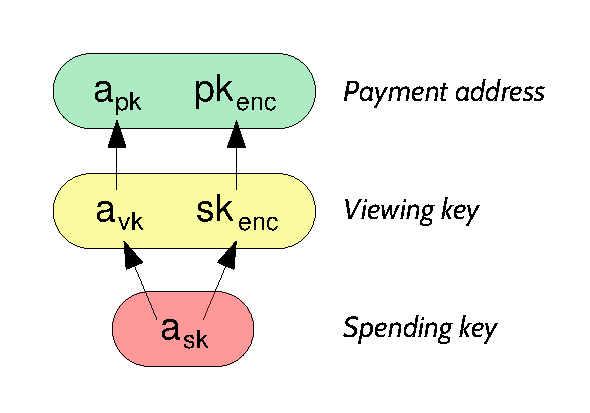
\includegraphics[scale=.8]{key_components}
\end{center}

Note that a \spendingKey holder can derive the other components\changed{,
and a \viewingKey holder can derive $(\AuthPublic, \TransmitPublic)$,}
even though these components are not formally part of the respective keys.
Implementations \MAY cache these derived components, provided that
they are deleted if the corresponding source component is deleted.

The composition of \paymentAddresses\changed{, \viewingKeys,} and \spendingKeys
is a cryptographic protocol detail that should not normally be
exposed to users. However, user-visible operations should be provided
to:

\begin{itemize}
\changed{
  \item obtain a \paymentAddress from a \viewingKey; and
}
  \item obtain a \paymentAddress\changed{ or \viewingKey} from a \spendingKey.
\end{itemize}

\changed{$\AuthPrivate$ and $\DiscloseKey$ are each 252 bits.}
$\AuthPublic$, $\TransmitPrivate$, and $\TransmitPublic$, are each 256 bits.

\changed{
$\DiscloseKey$, $\AuthPublic$, $\TransmitPrivate$, and $\TransmitPublic$ are
derived as follows:

\begin{equation*}
\begin{aligned}
\DiscloseKey &:= \Trailing{252}(\PRFaddr{\AuthPrivate}(0)) & \hspace{30em} \\
\AuthPublic &:= \PRFaddr{\DiscloseKey}(1) & \\
\TransmitPrivate &:= \Clamp(\PRFaddr{\AuthPrivate}(2)) & \\
\TransmitPublic &:= \CurveMultiply(\TransmitPrivate)
\end{aligned}
\end{equation*}

where $\Clamp$ performs the clamping of Curve25519 private key bits, and
$\CurveMultiply$ performs point multiplication, both as defined in \cite{Curve25519}.
}

Users can accept payment from multiple parties with a single
$\PaymentAddress$ and the fact that these payments are destined to
the same payee is not revealed on the blockchain, even to the
paying parties. \emph{However} if two parties collude to compare a
$\PaymentAddress$ they can trivially determine they are the same. In the
case that a payee wishes to prevent this they should create a distinct
\paymentAddress for each payer.

\subsection{Coins}

A \coin (denoted $\Coin{}$) is a tuple $\changed{(\AuthPublic, \Value,
\CoinAddressRand, \CoinCommitRand)}$ which represents that a value $\Value$ is
spendable by the recipient who holds the $\authKeypair$ key pair
$(\AuthPublic, \AuthPrivate)$ such that
$\AuthPublic = \PRFaddr{\AuthPrivate}(0)$.
 
\begin{itemize}
    \item $\AuthPublic$ is a 32-byte \authKeypair public key of the recipient.
    \item $\Value$ is a 64-bit unsigned integer representing the value of the
        \coin in \zatoshi (1 \ZEC = $10^8$ \zatoshi).
    \item $\CoinAddressRand$ is a 32-byte $\PRFsn{\AuthPrivate}$ preimage.
    \item $\CoinCommitRand$ is a 48-byte \COMMtrapdoor.
\end{itemize}

$\CoinCommitRand$ is randomly generated by the sender. \changed{$\CoinAddressRand$
is generated from a random seed $\CoinAddressPreRand$ using
$\PRFrho{\CoinAddressPreRand}$.} Only a commitment to these values is disclosed
publicly, which allows the tokens $\CoinCommitRand$ and $\CoinAddressRand$ to blind
the value and recipient \emph{except} to those who possess these tokens.

Note that the value $\CoinCommitS$ described as being part of a \coin in the
\Zerocash paper \cite{ZerocashOakland} is not encoded because the instantiation
of $\COMM{\CoinCommitS}$ does not use it.

\subsubsection{Coin Commitments}

The underlying $\Value$ and $\AuthPublic$ are blinded with $\CoinAddressRand$
and $\CoinCommitRand$ using the collision-resistant hash function \changed{$\FullHash$}.
The resulting hash $\cm = \CoinCommitment(\Coin{})$.

\newsavebox{\cmbox}
\begin{lrbox}{\cmbox}
\setchanged
\begin{bytefield}[bitwidth=0.040em]{840}
        \bitbox{80}{$\CoinCommitmentLeadByte$} &
	\bitbox{256}{256 bit $\AuthPublic$} &
	\bitbox{128}{64 bit $\Value$} &
	\bitbox{256}{256 bit $\CoinAddressRand$}
	\bitbox{256}{256 bit $\CoinCommitRand$} &
\end{bytefield}
\end{lrbox}

\changed{
\hskip 2em $\cm := \FullHashbox{\cmbox}$
}

\subsubsection{Serial numbers}

A \serialNumber (denoted $\sn$) equals 
$\PRFsn{\AuthPrivate}(\CoinAddressRand)$. A \coin is spent by proving
knowledge of $\CoinAddressRand$ and $\AuthPrivate$ in zero knowledge while
disclosing $\sn$, allowing $\sn$ to be used to prevent double-spending.

\subsubsection{Coin plaintexts and memo fields}

Transmitted coins are stored on the blockchain in encrypted form, together with
a \coinCommitment $\cm$.

The \coinPlaintexts associated with a \PourDescription are encrypted to the
respective \transmitKeypair keys $\TransmitPublicNew{\mathrm{1}..\NNew}$,
and the result forms part of a \coinsCiphertext (see section
``In-band secret distribution'' for further details).

Each \coinPlaintext (denoted $\CoinPlaintext{}$) consists of
$(\changed{\AuthPublic,\;}\Value, \CoinAddressRand, \CoinCommitRand\changed{, \Memo})$.

The first \changed{four} of these fields are as defined earlier.
\changed{$\Memo$ is a 64-byte \memo associated with this \coin.

The usage of the $\memo$ is by agreement between the sender and recipient of the
\coin. It should be encoded as a UTF-8 human-readable string \cite{Unicode}, padded
with zero bytes. Wallet software is expected to strip any trailing zero bytes and
then display the resulting UTF-8 string to the recipient user, where applicable.
Incorrect UTF-8-encoded byte sequences should be displayed as replacement characters
(\ReplacementCharacter). This does not preclude uses of the \memo by automated
software, but specification of such usage is not in the scope of this document.
}

\subsection{Coin Commitment Tree}

\begin{center}
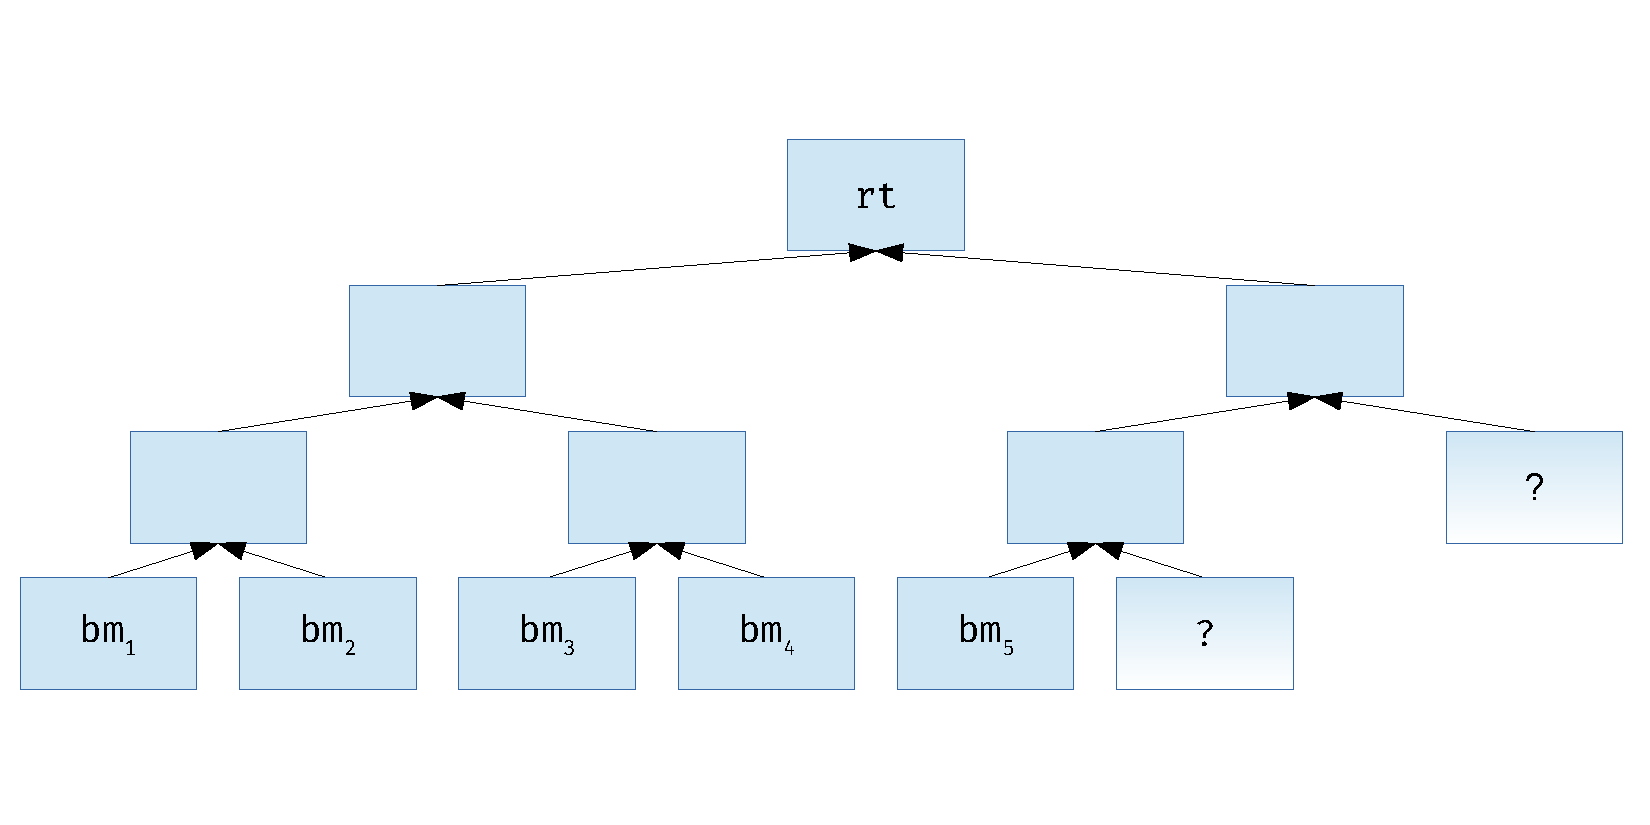
\includegraphics[scale=.4]{incremental_merkle}
\end{center}

The \coinCommitmentTree is an \incrementalMerkleTree of depth $\MerkleDepth$ used to
store \coinCommitments that \PourTransfers produce. Just as the \term{unspent
transaction output set} (UTXO) used in Bitcoin, it is used to express the existence
of value and the capability to spend it. However, unlike the UTXO, it is \emph{not}
the job of this tree to protect against double-spending, as it is append-only.

Blocks in the blockchain are associated (by all nodes) with the root of this tree
after all of its constituent \PourDescriptions' \coinCommitments have been
entered into the tree associated with the previous block.

\subsection{Spent Serials Map}

Transactions insert \serialNumbers into a \spentSerialsMap which is maintained 
alongside the UTXO by all nodes.

\eli{a tx is just a string, so it doesn't insert anything. Rather, nodes process 
tx's and the ``good'' ones lead to the addition of serials to the spent serials 
map.}

Transactions that attempt to insert a \serialNumber into this map that already
exists within it are invalid as they are attempting to double-spend.

\eli{After defining \term{transaction}, one should define what a \term{legal tx} is
(this definition depends on a particular blockchain [view]) and only then can one
talk about ``attempts'' of transactions, and insertions of serial numbers into the
spent serials map.}

\subsection{The Blockchain}

At a given point in time, the \blockchainview of each \fullnode consists of a
sequence of one or more valid \blocks. Each \block consists of a sequence of one or
more \transactions. In a given node's \blockchainview, \treestates are chained in an
obvious way:

\begin{itemize}
  \item The input \treestate of the first \block is the empty \treestate.
  \item The input \treestate of the first \transaction of a \block is the final
        \treestate of the immediately preceding \block.
  \item The input \treestate of each subsequent \transaction in a \block is the
        output \treestate of the immediately preceding \transaction.
  \item The final \treestate of a \block is the output \treestate of its last
        \transaction.
\end{itemize}

An \anchor is a Merkle tree root of a \treestate, and uniquely identifies that
\treestate given the assumed security properties of the Merkle tree's hash function.

Each \transaction is associated with a \sequenceOfPourDescriptions.
\todo{They also have a transparent value flow that interacts with the Pour
\changed{$\vpubOld$ and} $\vpubNew$.}
Inputs and outputs are associated with a value.

The total value of the outputs must not exceed the total value of the inputs.

The \anchor of the \changed{first} \PourDescription in a \transaction must refer to
some earlier \block's final \treestate.

\changed{
The \anchor of each subsequent \PourDescription may refer either to some earlier
\block's final \treestate, or to the output \treestate of the immediately preceding
\PourDescription.
}

These conditions act as constraints on the blocks that a \fullnode will
accept into its \blockchainview.

We rely on Bitcoin-style consensus for \fullnodes to eventually converge on their 
views of valid \blocks, and therefore of the sequence of \treestates in those 
\blocks.


\subparagraph{Value pool}

Transaction inputs insert value into a \term{value pool}, and transaction outputs 
remove value from this pool. The remaining value in the pool is available to miners 
as a fee.

\section{Pour Transfers and Descriptions}

A \PourDescription is data included in a \block that describes a \PourTransfer,
i.e. a confidential value transfer. This kind of value transfer is the primary
\Zerocash-specific operation performed by transactions; it uses, but should not be
confused with, the \PourCircuit used for the \zkSNARK proof and verification.

A \PourTransfer spends $\NOld$ \coins $\cOld{1..\NOld}$ and creates $\NNew$ \coins
$\cNew{1..\NNew}$. \Zcash transactions have an additional field $\vpour$, which is
a \sequenceOfPourDescriptions.

Each \PourDescription consists of:

\begin{list}{}{}
\changed{
\item $\vpubOldField$ which is a value $\vpubOld$ that the \PourTransfer removes
from the value pool.
}

\item $\vpubNewField$ which is a value $\vpubNew$ that the \PourTransfer inserts
into the value pool.

\item $\anchorField$ which is a merkle root $\rt$ of the \coinCommitmentTree at
some block height in the past, or the merkle root produced by a previous pour in
this transaction. \sean{We need to be more specific here.}

\item $\scriptSig$ which is a \script that creates conditions for acceptance of a
\PourDescription in a transaction.

\item $\scriptPubKey$ which is a \script used to satisfy the conditions of the
$\scriptSig$.

\item $\serials$ which is an $\NOld$ size sequence of serials $\snOld{\mathrm{1}..\NOld}$.

\item $\commitments$ which is a $\NNew$ size sequence of \coinCommitments 
$\cmNew{\mathrm{1}..\NNew}$.

\changed{
\item $\ephemeralKey$ which is a Curve25519 public key $\EphemeralPublic$.

\item $\encCiphertexts$ which is a $\NNew$ size sequence of ciphertext
components, $\TransmitCiphertext{\mathrm{1}..\NNew}$.

\item $\discloseCiphertexts$ which is a $\NOld$ size sequence of ciphertext
components, $\DiscloseCiphertext{\mathrm{1}..\NOld}$.

\item $\sharedCiphertext$ which is the ciphertext component
$\SharedCiphertext$.

(The preceding four fields together form the \coinsCiphertext.)

\item $\randomSeed$ which is a random 256-bit seed $\RandomSeed$.
}

\item $\vmacs$ which is a $\NOld$ size sequence of message authentication tags
$\h{\mathrm{1}..\NOld}$ that bind $\hSig$ to each $\AuthPrivate$ of the
$\PourDescription$.

\item $\zkproof$ which is the zero-knowledge proof $\PourProof$.

\end{list}

\todo{Describe case where there are fewer than $\NOld$ real input coins.}

\subparagraph{Computation of $\hSig$}

\newsavebox{\hsigbox}
\begin{lrbox}{\hsigbox}
\setchanged
\begin{bytefield}[bitwidth=0.035em]{1064}
	\bitbox{80}{$\hSigInputVersionByte$} &
	\bitbox{256}{256 bit $\snOld{0}$} &
	\bitbox{24}{...} &
	\bitbox{256}{256 bit $\snOld{\NOld-1}$} &
	\bitbox{256}{$\RandomSeed$}
	\bitbox{256}{$\scriptPubKey$}
\end{bytefield}
\end{lrbox}

\changed{
Given a \PourDescription, we define:

\hskip 2em $\hSig := \FullHashbox{\hsigbox}$
}

\subparagraph{Merkle root validity}

A \PourDescription is valid if $\rt$ is a \coinCommitmentTree root found in 
either the blockchain or a merkle root produced by inserting the \coinCommitments 
of a previous $\PourDescription$ in the transaction to the \coinCommitmentTree 
identified by that previous $\PourDescription$'s $\anchor$.

\subparagraph{Non-malleability}

A \PourDescription is valid if the script formed by appending $\scriptPubKey$ to 
$\scriptSig$ returns $true$. The $\scriptSig$ is cryptographically bound to 
$\PourProof$.

\subparagraph{Balance}

A \PourTransfer can be seen, from the perspective of the transaction, as
an input \changed{and an output simultaneously}.
\changed{$\vpubOld$ takes value from the value pool and}
$\vpubNew$ adds value to the value pool. As a result, \changed{$\vpubOld$ is
treated like an \emph{output} value, whereas} $\vpubNew$ is treated like an
\emph{input} value.

\changed{
Note that unlike original \Zerocash \cite{ZerocashOakland}, \Zcash does not have
a distinction between Mint and Pour transfers. The addition of $\vpubOld$ to a
\PourDescription subsumes the functionality of Mint. Also, \PourDescriptions
are indistinguishable regardless of the number of real input \coins.
}

\subparagraph{Commitments and Serials}

A \transaction that contains one or more \PourDescriptions, when entered into the 
blockchain, appends to the \coinCommitmentTree with all constituent 
\coinCommitments. All of the constituent \serialNumbers are also entered into the 
\spentSerialsMap of the \blockchainview \emph{and} \mempool. A \transaction is not 
valid if it attempts to add a \serialNumber to the \spentSerialsMap that already 
exists in the map.

\subsection{Pour Circuit and Proofs}

In \Zcash, $\NOld$ and $\NNew$ are both $2$.

A valid instance of $\PourProof$ assures that given a \term{primary input}:

\begin{itemize}
  \item[] $(\rt, \snOld{\mathrm{1}..\NOld}, \cmNew{\mathrm{1}..\NNew}, \changed{\vpubOld,\;}
\vpubNew, \hSig, \h{1..\NOld}, \changed{\TransmitCiphertext{1..\NNew},
\DiscloseCiphertext{1..\NOld}, \SharedCiphertext})$,
\end{itemize}

there exists a witness of \term{auxiliary input}:

\begin{itemize}
  \item[] $(\treepath{1..\NOld}, \cOld{1..\NOld}, \AuthPrivateOld{\mathrm{1}..\NOld},
\changed{\DiscloseKeyOld{\mathrm{1}..\NOld}, \cpNew{1..\NNew},
\CoinAddressPreRand, \TransmitKey{1..\NNew}, \DerivedKey{1..\NOld}, \SharedKey{},
\TransmitPublicNew{\mathrm{1}..\NNew}, \EphemeralPrivate})$
\end{itemize}

where:

\begin{itemize}
  \item[] for each $i \in \{1..\NOld\}$: $\cOld{i}$ = $(\AuthPublicOld{i},
\vOld{i}, \CoinAddressRandOld{i}, \CoinCommitRandOld{i})$;
  \item[] for each $i \in \{1..\NNew\}$: $\cpNew{i}$ = $(\AuthPublicNew{i},
\vNew{i}, \CoinAddressRandNew{i}, \CoinCommitRandNew{i}, \Memo_i)$,
and $\TransmitPlaintext{i}$ is a raw encoding of $\cpNew{i}$;
\end{itemize}

such that the following conditions hold:

\subparagraph{Merkle path validity}

for each $i \in \{1..\NOld\}$ \changed{$\mid$ $\vOld{i} \neq 0$}:
$\treepath{i}$ must be a valid path of depth $\MerkleDepth$ from \linebreak
$\CoinCommitment(\cOld{i})$ to \coinCommitmentTree root $\rt$.

\subparagraph{Balance}

$\changed{\vpubOld\; +} \vsum{i=1}{\NOld} \vOld{i} = \vpubNew + \vsum{i=1}{\NNew} \vNew{i}$.

\subparagraph{Serial integrity}

for each $i \in \{1..\NNew\}$: 
$\snOld{i} = \PRFsn{\AuthPrivateOld{i}}(\CoinAddressRandOld{i})$.

\subparagraph{Spend authority}

for each $i \in \{1..\NOld\}$:
\changed{
$\DiscloseKeyOld{i} = \PRFaddr{\AuthPrivateOld{i}}(0)$ and
$\AuthPublicOld{i} = \PRFaddr{\DiscloseKeyOld{i}}(1)$.
}

\subparagraph{Non-malleability}

for each $i \in \{1..\NOld\}$:
$\h{i} = \PRFpk{\AuthPrivateOld{i}}(i, \hSig)$.

\changed{
\subparagraph{Uniqueness of $\CoinAddressRandNew{i}$}

for each $i \in \{1..\NNew\}$:
$\CoinAddressRandNew{i} = \PRFrho{\CoinAddressPreRand}(i, \hSig)$.
}

\subparagraph{Commitment integrity}

for each $i \in \{1..\NNew\}$: $\cmNew{i}$ = $\CoinCommitment(\cNew{i})$.

\changed{
\subparagraph{$\TransmitCiphertext{}$ integrity}

for each $i \in \{1..\NNew\}$:
$\TransmitCiphertext{i} = \SymEncrypt{\TransmitKey{i}}(\TransmitPlaintext{i})$.

\subparagraph{$\DiscloseCiphertext{}$ integrity}

for each $i \in \{1..\NOld\}$:
$\DiscloseCiphertext{i} = \SymEncrypt{\DerivedKey{i}}(\SharedKey{})$
and $\DerivedKey{i} = \PRFdk{\DiscloseKeyOld{i}}(i, \hSig)$.
}

\subparagraph{\changed{$\SharedCiphertext$ integrity}}

\newsavebox{\sharedbox}
\begin{lrbox}{\sharedbox}
\setchanged
\begin{bytefield}[bitwidth=0.045em]{512}
    \bitbox{256}{256 bit $\TransmitKey{\mathrm{1}}$} &
    \bitbox{40}{...} &
    \bitbox{256}{256 bit $\TransmitKey{\NNew}$} \\
    \bitbox{256}{256 bit $\TransmitPublicNew{\mathrm{1}}$} &
    \bitbox{40}{...} &
    \bitbox{256}{256 bit $\TransmitPublicNew{\NNew}$} \\
    \bitbox{256}{256 bit $\EphemeralPrivate$}
\end{bytefield}
\end{lrbox}

\changed{
$\SharedCiphertext = \SymEncrypt{\SharedKey{}}(\SharedPlaintext{})$

where $\SharedPlaintext{} = \Justthebox{\sharedbox}{-9.5ex}$
}

\section{In-band secret distribution}

In order to transmit the secret $\Value$, $\CoinAddressRand$, and $\CoinCommitRand$
(necessary for the recipient to later spend) \changed{and also a \memo} to the
recipient \emph{without} requiring an out-of-band communication channel, the
\transmitKeypair public key $\TransmitPublic$ is used to encrypt these
secrets. The recipient's possession of the associated
$(\PaymentAddress, \SpendingKey)$ (which contains both $\AuthPublic$ and
$\TransmitPrivate$) is used to reconstruct the original \coin \changed{ and \memo}.

\changed{Several more encryptions are used to also reveal these values to a
holder of a \viewingKey for any of the input \coins, and also to permit them
to check whether the other encryptions are valid.}

All of the resulting ciphertexts are combined to form a \coinsCiphertext.

\newsavebox{\kdfbox}
\begin{lrbox}{\kdfbox}
\setchanged
\begin{bytefield}[bitwidth=0.032em]{832}
    \bitbox{256}{256 bit $\DHSecret{i}$} &
    \bitbox{256}{256 bit $\EphemeralPublic$} &
    \bitbox{256}{256 bit $\TransmitPublicNew{i}$} &
    \bitbox{160}{8 bit $i-1$}
\end{bytefield}
\end{lrbox}

\subsection{Encryption}

\changed{
Let $\SymEncrypt{\Key}(\Plaintext)$ be the $\SymSpecific$ \cite{rfc7539}
encryption of plaintext $\Plaintext$ with empty ``additional data", all-zero nonce,
and key $\Key$.

Similarly, let $\SymDecrypt{\Key}(\Ciphertext)$ be the $\SymSpecific$
decryption of ciphertext $\Ciphertext$ with empty ``additional data", all-zero
nonce, and key $\Key$. The result is either the plaintext byte sequence,
or $\bot$ indicating failure to decrypt.

Define:

$\KDF(\DHSecret{i}, \EphemeralPublic, \TransmitPublicNew{i}, i) := \FullHashbox{\kdfbox}$.
}

Let $\TransmitPublicNew{\mathrm{1}..\NNew}$ be the \changed{Curve25519} public keys
for the intended recipient addresses of each new \coin,
\changed{let $\DiscloseKeyOld{\mathrm{1}..\NOld}$ be the \discloseKey for each of
the addresses from which the old \coins are sent,} and let $\CoinPlaintext{1..\NNew}$
be the \coinPlaintexts.
Let $\TransmitPlaintext{i}$ be the raw encoding of $\CoinPlaintext{i}$.

Then to encrypt:

\begin{itemize}
\changed{
  \item Let $\SharedPlaintext{} := \Justthebox{\sharedbox}{-9.5ex}$
  \item Generate a new Curve25519 (public, private) key pair
$(\EphemeralPublic, \EphemeralPrivate)$, and a new $\SymSpecific$ key $\SharedKey{}$.
  \item For $i$ in $\{1..\NNew\}$,
    \begin{itemize}
      \item Let $\DHSecret{i} := \CurveMultiply(\TransmitPublicNew{i},
\EphemeralPrivate)$.
      \item Let $\TransmitKey{i} := \KDF(\DHSecret{i}, \EphemeralPublic,
\TransmitPublicNew{i}, i)$.
      \item Let $\TransmitCiphertext{i} :=
\SymEncrypt{\TransmitKey{i}}(\TransmitPlaintext{i})$.
    \end{itemize}
  \item For $i$ in $\{1..\NOld\}$,
    \begin{itemize}
      \item Let $\DerivedKey{i} := \PRFdk{\DiscloseKeyOld{i}}(i, \hSig)$.
      \item Let $\DiscloseCiphertext{i} := \SymEncrypt{\DerivedKey{i}}(\SharedKey{})$.
    \end{itemize}
  \item Let $\SharedCiphertext := \SymEncrypt{\SharedKey{}}(\SharedPlaintext{})$.
}
\end{itemize}

The resulting \coinsCiphertext is $\changed{(\EphemeralPublic,
\TransmitCiphertext{\mathrm{1}..\NNew}, \DiscloseCiphertext{\mathrm{1}..\NOld},
\SharedCiphertext)}$.

\subsection{Decryption by a Recipient}

Let $(\TransmitPublic, \TransmitPrivate)$ be the recipient's \changed{Curve25519}
(public, private) key pair, and let $\cmNew{\mathrm{1}..\NNew}$ be the coin
commitments of each output coin. Then for each $i$ in $\{1..\NNew\}$, the recipient
will attempt to decrypt that ciphertext component as follows:

\changed{
\begin{itemize}
  \item Let $\DHSecret{i} := \CurveMultiply(\EphemeralPublic, \TransmitPrivate)$.
  \item Let $\TransmitKey{i} := \KDF(\DHSecret{i}, \EphemeralPublic,
\TransmitPublicNew{i}, i)$.
  \item Return $\DecryptCoin(\TransmitKey{i}, \TransmitCiphertext{i}, \cmNew{i}).$
\end{itemize}

$\DecryptCoin(\TransmitKey{i}, \TransmitCiphertext{i}, \cmNew{i})$ is defined as follows:

\begin{itemize}
  \item Let $\TransmitPlaintext{i} :=
\SymDecrypt{\TransmitKey{i}}(\TransmitCiphertext{i})$.
  \item If $\TransmitPlaintext{i} = \bot$, return $\bot$.
  \item Extract $\CoinPlaintext{i} = (\AuthPublicNew{i}, \ValueNew{i},
\CoinAddressRandNew{i}, \CoinCommitRandNew{i}, \Memo_i)$ from $\TransmitPlaintext{i}$.
  \item If $\CoinCommitment((\AuthPublicNew{i}, \ValueNew{i}, \CoinAddressRandNew{i},
\CoinCommitRandNew{i})) \neq \cmNew{i}$, return $\bot$, else return $\CoinPlaintext{i}$.
\end{itemize}
}

Note that this corresponds to step 3 (b) i. and ii. (first bullet point) of the
$\Receive$ algorithm shown in Figure 2 of \cite{ZerocashOakland}.

To test whether a \coin is unspent in a particular \blockchainview also requires
the \authKeypair private key $\AuthPrivate$; the coin is unspent if and only if
$\sn = \PRFsn{\AuthPrivate}(\CoinAddressRand)$ is not in the \spentSerials
for that \blockchainview.

Note that a coin may change from being unspent to spent on a given \blockchainview,
as transactions are added to that view. Also, blockchain reorganisations may cause
the transaction in which a coin was output to no longer be on the consensus
blockchain.

\changed{
\subsection{Decryption by a Viewing Key Holder}

Let $\DiscloseKey{}$ be a \viewingKey holder's \discloseKey.
Then for each \PourDescription in its \blockchainview, the \viewingKey holder
will attempt to decrypt the corresponding \coinsCiphertext as follows:

\begin{enumerate}
  \item Set $\SharedPlaintext{} := \bot$.
  \item For $i$ in $\{1..\NNew\}$,
    \begin{itemize}
      \item Let $\DerivedKey{i} := \PRFdk{\DiscloseKey{}}(i, \hSig)$.
      \item Let $\SharedKey{i} := \SymDecrypt{\DerivedKey{i}}(\DiscloseCiphertext{i})$.
      \item If $\SharedKey{i} = \bot$ then continue with the next $i$.
      \item Let $\SharedPlaintext{i} := \SymDecrypt{\SharedKey{i}}(\SharedCiphertext)$.
      \item If $\SharedPlaintext{i} = \bot$ then continue with the next $i$.
      \item Set $\SharedPlaintext{} := \SharedPlaintext{i}$ and exit the loop.
    \end{itemize}
  \item If $\SharedPlaintext{} = \bot$ (i.e. it was not set in the loop), then this
transaction does not contain any information decryptable by the \viewingKey; set
$\CoinPlaintext{i} = \bot$ for $i$ in $\{1..\NNew\}$ and return
$\CoinPlaintext{\mathrm{1}..\NNew}$.
  \item Extract $\TransmitKey{1..\NNew}$, $\TransmitPublicNew{\mathrm{1}..\NNew}$,
and $\EphemeralPrivate$ from $\SharedPlaintext{}$.
  \item For $i$ in $\{1..\NNew\}$,
    \begin{itemize}
      \item Let $\CoinPlaintext{i} :=
\DecryptCoin(\TransmitKey{i}, \TransmitCiphertext{i}, \cmNew{i})$.
      \item Let $\DHSecret{i} := \CurveMultiply(\TransmitPublicNew{i}, \EphemeralPrivate)$.
      \item Let $\TransmitKeyCompare{i} := \KDF(\DHSecret{i}, \EphemeralPublic,
\TransmitPublicNew{i}, i)$.
      \item If $\CoinPlaintext{i} \neq \bot$ and
$\TransmitKeyCompare{i} \neq \TransmitKey{i}$ then set the \memo
of $\CoinPlaintext{i}$ to be $\bot$ (indicating that, although this is a valid
coin, the recipient would not have been able to decrypt it, and that the \memo
cannot be verified).
    \end{itemize}
  \item Return $\CoinPlaintext{\mathrm{1}..\NNew}$.
\end{enumerate}

If a party holds more than one \viewingKey, it may optimize the above
procedure by performing the loop in step 2 for the $\DiscloseKey{}$ of each
\viewingKey. It may be assumed that the first $\SharedPlaintext{i}$ that
decrypts correctly is the one that should be used in step 4 onward.
(However, additional information is provided by which \viewingKey was able
to decrypt each $\DiscloseCiphertext{i}$.)

The public key encryption used in this part of the protocol is based loosely on
other encryption schemes based on Diffie-Hellman over an elliptic curve, such
as ECIES or the $\CryptoBoxSeal$ algorithm defined in libsodium \cite{cryptoboxseal}.
Note that:
\begin{itemize}
  \item The same ephemeral key is used for all encryptions to the recipient keys
        in a given \PourDescription.
  \item In addition to the Diffie-Hellman secret, the KDF takes as input the
        public keys of both parties, and the index $i$.
  \item The nonce parameter to $\SymSpecific$ is not used.
  \item The ephemeral secret $\EphemeralPrivate$ is included together with
        the \transmitKeypair public keys of the recipients, symmetrically
        encrypted to the \discloseKey.
        This allows a \viewingKey holder to check whether the
        indicated recipients would be able to decrypt a given component, and
        if so to decrypt the memo field. (We do not rely on this to ensure
        that a \viewingKey holder can decrypt the other components of the
        output coins; instead, those are symmetrically encrypted to the
        \viewingKey and the correctness of this encryption is checked by the
        \PourCircuit.)
\end{itemize}
}


\section{Encoding Addresses, Keys, Coin plaintexts, and Pour descriptions}

This section describes how \Zcash encodes \paymentAddresses, \spendingKeys,
\viewingKeys, \coinPlaintexts, and \PourDescriptions.

Addresses, keys, and coins, can be encoded as a byte string; this is called
the \term{raw encoding}. This byte string can then be further encoded using
Base58Check. The Base58Check layer is the same as for upstream \Bitcoin
addresses \cite{Base58Check}.

SHA-256 compression function outputs are always represented as strings of 32
bytes.

The language consisting of the following encoding possibilities is prefix-free.

\subsection{Transparent Payment Addresses}

These are encoded in the same way as in \Bitcoin \cite{Base58Check}.

\subsection{Transparent Private Keys}

These are encoded in the same way as in \Bitcoin \cite{Base58Check}.

\subsection{Private Payment Addresses}

A \paymentAddress consists of $\AuthPublic$ and $\TransmitPublic$.
$\AuthPublic$ is a SHA-256 compression function output.
$\TransmitPublic$ is a \changed{Curve25519} public key, for use with the
encryption scheme defined in section ``In-band secret distribution".

\subsubsection{Raw Encoding}

The raw encoding of a \paymentAddress consists of:

\begin{equation*}
\begin{bytefield}[bitwidth=0.07em]{520}
\changed{
    \bitbox{48}{$\SpendingKeyLeadByte$}
  &}\bitbox{256}{256 bit $\AuthPublic$} &
    \bitbox{256}{\changed{256 bit} $\TransmitPublic$}
\end{bytefield}
\end{equation*}

\begin{itemize}
\changed{
    \item A byte, $\PaymentAddressLeadByte$, indicating this version of the
        raw encoding of a \Zcash public address.
}
    \item 256 bits specifying $\AuthPublic$.
    \item \changed{256 bits} specifying $\TransmitPublic$, \changed{using the
        normal encoding of a Curve25519 public key \cite{Curve25519}}.
\end{itemize}

\daira{check that this lead byte is distinct from other Bitcoin stuff,
and produces `z' as the Base58Check leading character.}

\nathan{what about the network version byte?}

\subsection{Spending Keys}

A \spendingKey consists of $\AuthPrivate$.

\subsubsection{Raw Encoding}

The raw encoding of a \spendingKey consists of, in order:

\begin{equation*}
\begin{bytefield}[bitwidth=0.07em]{264}
\changed{
    \bitbox{48}{$\SpendingKeyLeadByte$}
    \bitbox{24}{$0^4$} &
  &}\bitbox{252}{\changed{252} bit $\AuthPrivate$}
\end{bytefield}
\end{equation*}

\begin{itemize}
\changed{
    \item A byte $\SpendingKeyLeadByte$ indicating this version of the
        raw encoding of a \Zcash \spendingKey.
    \item 4 zero padding bits.
}
    \item \changed{252} bits specifying $\AuthPrivate$.
\end{itemize}

Note that, consistent with big-endian encoding, the zero padding occupies
the high-order 4 bits of the second byte.

\daira{check that this lead byte is distinct from other Bitcoin stuff,
and produces a suitable Base58Check leading character.}

\nathan{what about the network version byte?}

\changed{
\subsection{Viewing Keys}

A \viewingKey consists of a \discloseKey $\DiscloseKey$, and a
\transmitKeypair private key $\TransmitPrivate$.

\subsubsection{Raw Encoding}

The raw encoding of a \viewingKey consists of, in order:
}

\begin{equation*}
\begin{bytefield}[bitwidth=0.07em]{520}
\setchanged
    \bitbox{48}{$\ViewingKeyLeadByte$} &
    \bitbox{24}{$0^4$} &
    \bitbox{252}{252 bit $\DiscloseKey$}
    \bitbox{256}{256 bit $\TransmitPrivate$}
\end{bytefield}
\end{equation*}

\changed{
\begin{itemize}
    \item A byte $\ViewingKeyLeadByte$ indicating this version of the
        raw encoding of a \Zcash \viewingKey.
    \item 4 zero padding bits.
    \item 252 bits specifying $\DiscloseKey$.
    \item 256 bits specifying $\TransmitPrivate$.
\end{itemize}

Note that, consistent with big-endian encoding, the zero padding occupies
the high-order 4 bits of the second byte.

\daira{check that this lead byte is distinct from other Bitcoin stuff,
and produces a suitable Base58Check leading character.}

\nathan{what about the network version byte?}
}

\subsection{Coin Plaintexts}

\subsubsection{Raw Encoding}

The raw encoding of a \coinPlaintext $(\AuthPublic, \Value, \CoinAddressRand,
\CoinCommitRand, \Memo)$ consists of, in order:

\begin{equation*}
\begin{bytefield}[bitwidth=0.032em]{1352}
\changed{
    \bitbox{88}{$\TransmitPlaintextVersionByte$}&
    \bitbox{256}{$\AuthPublic$ (32 bytes)}&
  &}\bitbox{168}{$\Value$ (8 bytes)} &
    \bitbox{256}{$\CoinAddressRand$ (32 bytes)} &
    \bitbox{256}{$\CoinCommitRand$ (32 bytes)} &
    \changed{\bitbox{512}{$\Memo$ (64 bytes)}}
\end{bytefield}
\end{equation*}

\begin{itemize}
\changed{
    \item A byte $\TransmitPlaintextVersionByte$ indicating this version of the raw 
encoding of a \coinPlaintext.
    \item 32 bytes specifying $\AuthPublic$.
}
    \item 8 bytes specifying a big-endian encoding of $\Value$.
    \item 32 bytes specifying $\CoinAddressRand$.
    \item 32 bytes specifying $\CoinCommitRand$.
\changed{
    \item 64 bytes specifying $\Memo$.
}
\end{itemize}


\section{Differences from the Zerocash paper}

\subsection{Unification of Mints and Pours}

\todo{}

\subsection{Faerie Gold attack and fix}

\todo{}

(The name ``Faerie Gold'' refers to various Celtic legends in which
faeries pay mortals in what appears to be gold, but which soon after
reveals itself to be leaves, gorse blossoms, gingerbread cakes, or
other less valuable things \cite{LG2004}.)

\subsection{Internal hash collision attack and fix}

The \Zerocash security proof requires that the composition of
$\COMM{\CoinCommitRand}$ and $\COMM{\CoinCommitS}$ is a computationally
binding commitment to its inputs $\AuthPublic$, $\Value$, and
$\CoinAddressRand$. However, the instantiation of $\COMM{\CoinCommitRand}$
and $\COMM{\CoinCommitS}$ in section 5.1 of the paper did not meet
the definition of a binding commitment at a 128-bit security level.
Specifically, the internal hash of $\AuthPublic$ and $\CoinAddressRand$
is truncated to 128 bits (motivated by providing statistical hiding
security). This allows an attacker, with a work factor on the order of
$2^{64}$, to find distinct values of $\CoinAddressRand$ with colliding
outputs of the truncated hash, and therefore the same \coinCommitment.
This would have allowed such an attacker to break the balance property
by double-spending coins, potentially creating arbitrary amounts of
currency for themself.

\Zcash uses a simpler construction with a single $\FullHash$ evaluation
for the commitment. The motivation for the nested construction in \Zerocash
was to allow Mint transactions to be publically verified without requiring
a ZK proof (as described under step 3 in section 1.3 of
\cite{ZerocashOakland}). Since \Zcash combines ``Mint'' and ``Pour''
transactions into a generalized Pour which always uses a ZK proof, it
does not require the nesting. A side benefit is that this reduces the
number of $\SHA$ evaluations needed to compute each \coinCommitment from
three to two, saving a total of four $\SHA$ evaluations in the
$\PourCircuit$.

Note that \Zcash coin commitments are not statistically hiding, and
so \Zcash does not support the ``everlasting anonymity'' property
described in section 8.1 of the \Zerocash paper \cite{ZerocashOakland},
even when used as described in that section. While it is possible to
define a statistically hiding, computationally binding commitment scheme
for this use at a 128-bit security level, the overhead of doing so
within the circuit was not considered to justify the benefits.

\subsection{Viewing keys}

\todo{}

\subsection{Changes to PRF inputs and truncation}

\todo{}

%The need for \Leading{253}{\CRH(.)} to be collision-resistant was not
%explicitly stated in \ (This does not follow from collision resistance of $\CRH$.)

\subsection{In-band secret distribution}

\todo{}

\subsection{Miscellaneous}

\begin{itemize}
    \item The paper defines a coin as a tuple $(\AuthPublic, \Value,
\CoinAddressRand, \CoinCommitRand, \CoinCommitS, \cm)$, whereas this specification
defines it as $(\AuthPublic, \Value, \CoinAddressRand, \CoinCommitRand)$.
This is just a clarification, because the instantiation of $\COMM{\CoinCommitS}$
in section 5.1 of the paper did not use $\CoinCommitS$ (and neither does the
new instantiation of $\CoinCommitment$). $\cm$ can be computed from the other
fields.
\end{itemize}


\section{Acknowledgements}

The inventors of \Zerocash are Eli Ben-Sasson, Alessandro Chiesa,
Christina Garman, Matthew Green, Ian Miers, Eran Tromer, and Madars
Virza.

The authors would like to thank everyone with whom they have discussed
the \Zerocash protocol design; in addition to the inventors, this includes
Mike Perry, Isis Lovecruft, Leif Ryge, Andrew Miller, Zooko Wilcox,
Nathan Wilcox, Samantha Hulsey, and no doubt others.

Mike Perry, Zooko Wilcox, and Nathan Wilcox contributed to the design
of selective transparency features, now called viewing keys.

The Faerie Gold attack was found by Zooko Wilcox.
The internal hash collision attack was found by Taylor Hornby.


\section{References}

\begingroup
\renewcommand{\section}[2]{}
\bibliographystyle{plain}
\bibliography{zcash}
\endgroup

\end{document}
